\section{Aufgabe 13}
\setcounter{section}{13}

Es seien $X = Y = \{1, 2, 3, 4 ,5\}$ und $f : X \rightarrow Y$ definiert durch

\begin{equation*}
    f(k) :=
    \begin{cases}
        k + 1,& \text{ falls } k \leq 4 \\
        1,    & \text{ falls } k =    5
    \end{cases}
\end{equation*}

\begin{enumerate}[(a)]
    \item Skizzieren Sie den Graph von $f$.
        \begin{figure}[h]
            \centering
            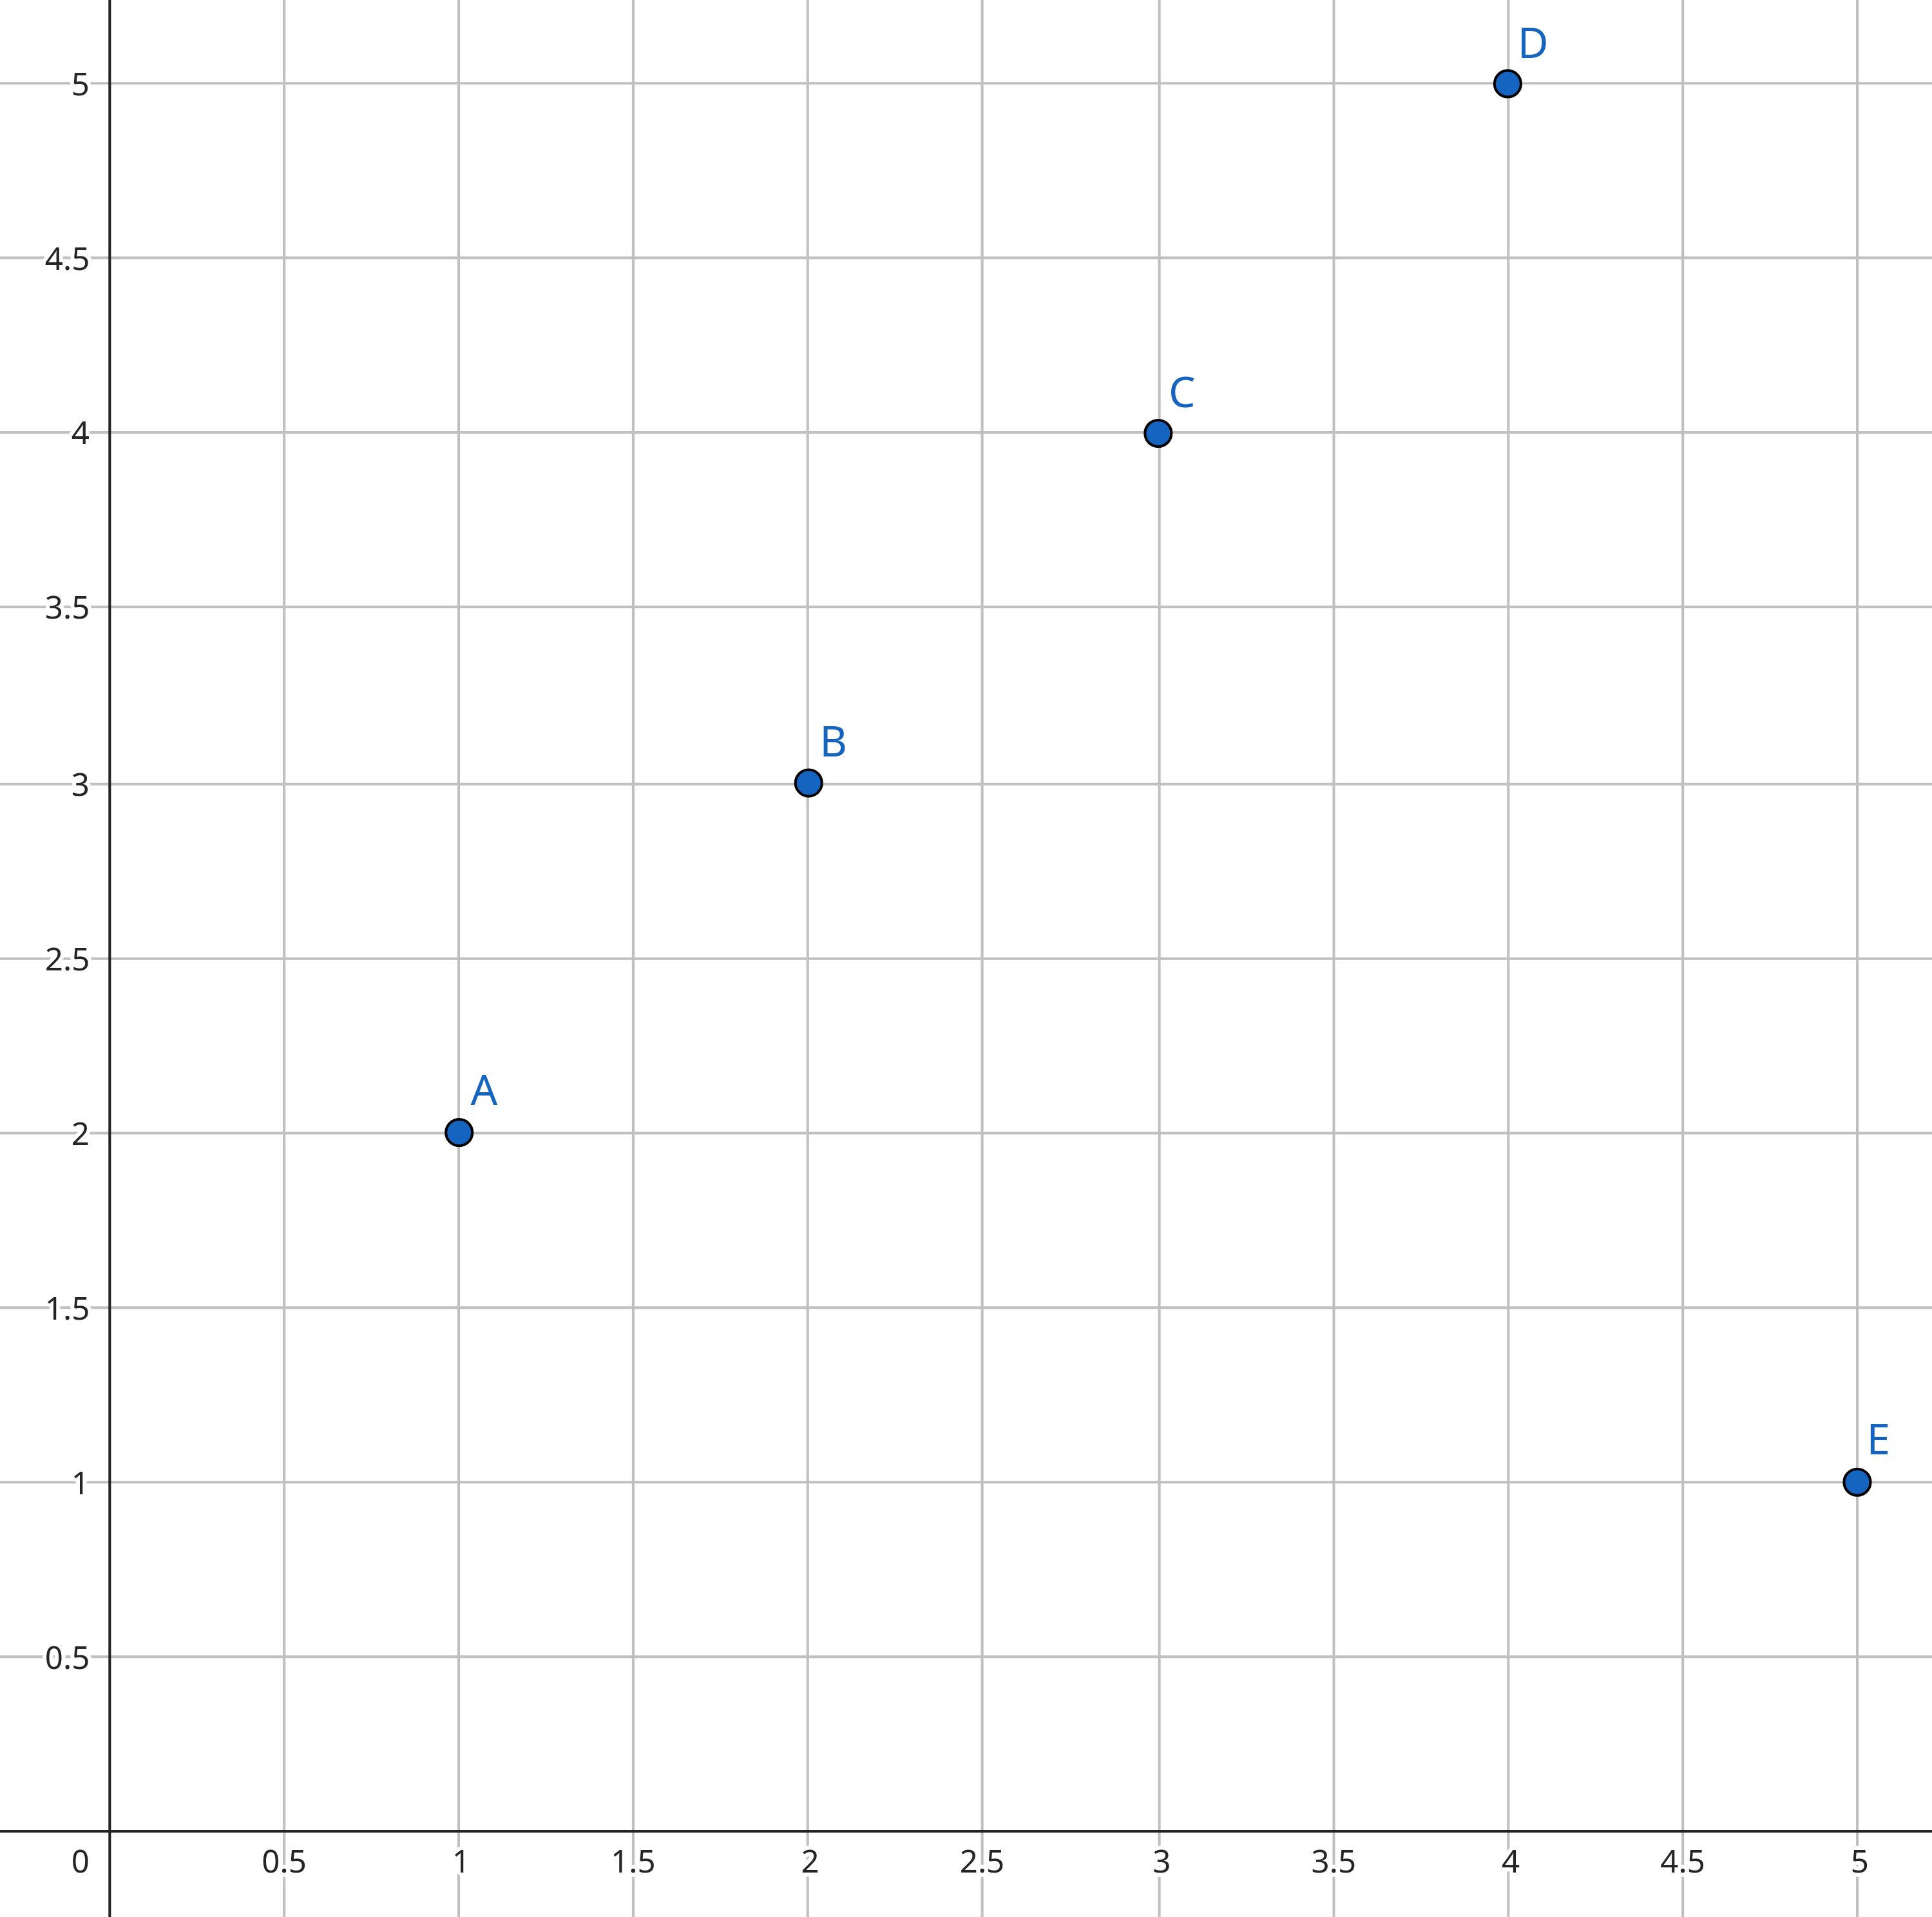
\includegraphics{./assets/abbildung-13-01.png}
            \caption{}
        \end{figure}

    \item Bestimmen Sie die Urbilder $f^{-1}(A)$, $f^{-1}(B)$, wobei $A := \{1,4\}$
        und $B := \{2,5\}$.

        \begin{equation*}
            \begin{aligned}
                f^{-1}(\{1, 4\}) &= \{x \in X : f(x) \in \{1, 4\}\} = \{3, 5\} \\[5pt]
                f^{-1}(\{2, 5\}) &= \{x \in X : f(x) \in \{2, 5\}\} = \{1, 4\}
            \end{aligned}
        \end{equation*}
\end{enumerate}
